\documentclass[t]{beamer}
\usetheme[deutsch]{KIT}
\setbeamercovered{transparent}
\setbeamertemplate{navigation symbols}{}

\KITfoot{YUV.KA - Praxis der Softwareentwicklung WS 11/12}
\usepackage[utf8]{inputenc}
\usepackage{ngerman}
\usepackage{verbatim}
\usenavigationsymbols

\title{YUV.KA}
\subtitle{Abschlusspräsentation Implementierungs- und Testphase}
%\author{Max Wagner $\cdot$ Patrick Gemander $\cdot$ Sebastian Ullrich $\cdot$ Michael Vollmer \\ Robert Hangu $\cdot$ Daniel Lebert}

\institute[ITEC]{Institut für Technische Informatik}

\TitleImage[trim = -20cm 0 0 0,height=\titleimageht]{images/logo.png}

\begin{document}

\begin{frame}
\maketitle
\end{frame}
 
\section{Architekturänderungen}
\begin{frame}
    \frametitle{Architekturänderungen}
    \noindent
    \begin{minipage}{3.5cm}
        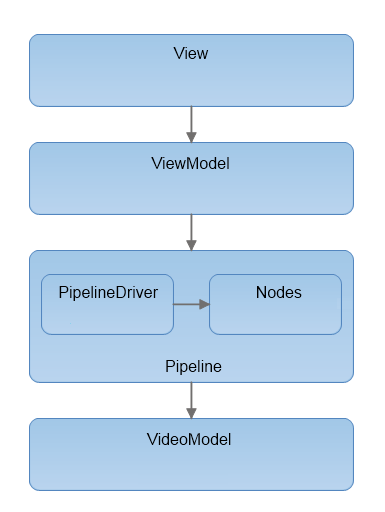
\includegraphics[scale=0.37]{images/Layers.png}
    \end{minipage}
    \hfill
    \begin{minipage}{8cm}
    \begin{itemize}
        \item Architektur größtenteils gleich
        \item Entwurf stellte sich als machbar heraus
        \item Änderungen bestehen größtenteils aus Implementationsdetails:
        \begin{itemize}
            \item Klassen, die nicht geplant werden konnten, da View-spezifisch
            \item Klassen, die nicht geplant werden konnten, da Framework-spezifisch
            \item Nicht vorhergesehene Properties und Methoden, die sich erst bei der Implementierung als notwendig herausgestellt haben
        \end{itemize}
    \end{itemize}
    \end{minipage}
\end{frame}

\begin{frame}
    \frametitle{Automatische Tests}
    \begin{itemize}
        \item Der größte Teil des Projektcodes wird abgedeckt.
        \item Die Aufbereitung der Daten für die View wird auf Korrektheit überprüft... \\
        die Darstellung dieser wird jedoch nicht abgedeckt, da die View keine Logik enthält.
        \item Die Korrektheit mancher Klassen können jedoch nicht automatisch verifiziert werden. \\
            Hier muss das Resultat manuell überprüft werden (bsp. YuvEncoder)
    \end{itemize}
\end{frame}

\begin{frame}
    \frametitle{Zeilenüberdeckung}
    \vspace{1cm}
\begin{tabular}{@{\extracolsep{\fill}} |l|c|}
\hline
Namespace &  Überdeckung in \% \\ \hline
YuvKA.Pipeline  &  98,32  \\ \hline
YuvKA.VideoModel  & 86,50 \\ \hline
YuvKA.ViewModel  & 92,77  \\ \hline
YuvKA.ViewModel.PropertyEditor  & 98,15  \\ \hline
YuvKA.Implementation  &  72,15 \\ \hline
YuvKA.Pipeline.Implementation  &  92,39  \\ \hline
YuvKA.ViewModel.Implementation  & 84,70 \\ \hline
YuvKA.ViewModel.PropertyEditor.Implementation  & 76,28  \\ \hline
\hline
\name{Overall} & 90,79 \\ \hline
\end{tabular}
~\\
Zeilen Testcode insgesamt: 3860
\end{frame}

\begin{frame}
    \frametitle{Globale Testfälle}
    Überprüfen das korrekte Zusammenspiel der einzelnen Programmschichten wie im Pflichtenheft spezifiziert: \\
    \begin{itemize}
        \item /T10/ Pipeline-Konstruktion
        \item /T20/ Manipulation einer Pipeline
        \item /T30/ Sicherung einer Pipeline
        \item /T40/ Videoverarbeitung
        \item /T50/ Videoanalyse
    \end{itemize}
    Dadurch dass wir die MVVM-Architektur verwenden, konnten diese Tests auch automatisiert werden.
\end{frame}

\begin{frame}
    \frametitle{Zeitplanung}
    Im Allgemeinen war die Zeitplanung für das Projekt akkurat, allerdings sind folgende Dinge aufgefallen:
    \begin{itemize}
        \item Die Produktivität während den Ferien war niedriger als erwartet.
        \item Der Einfluss anderer Veranstaltungen wurde unterschätzt.
        \item Die zum Debugging nötige Zeit wurde falsch kalkuliert.
    \end{itemize}
    \hspace{0.8cm}
    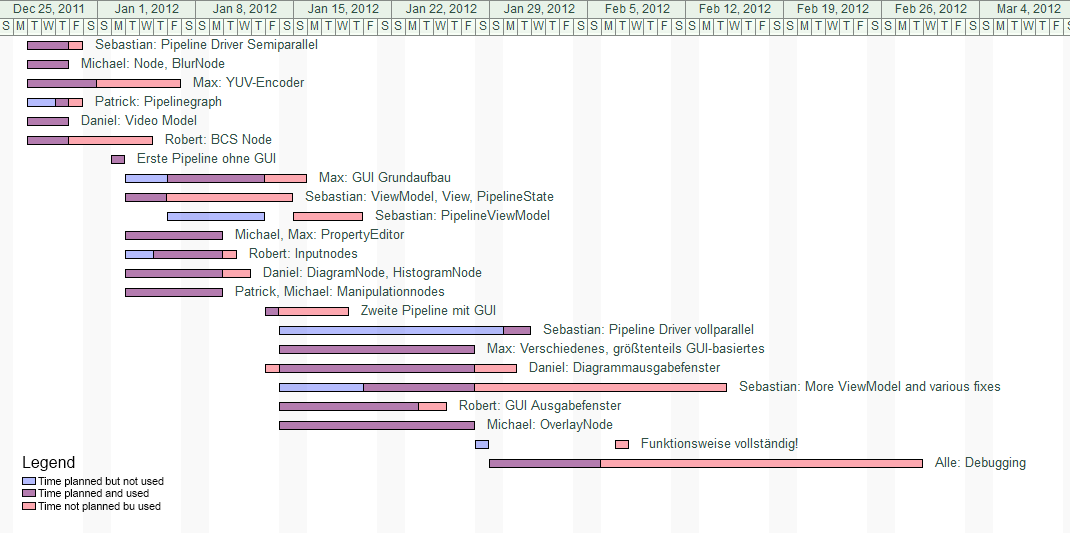
\includegraphics[scale=0.35]{images/gantt.png}
\end{frame}

\frame{
  \frametitle{Lizenzen}
  \center
  
\includegraphics[width=2em]{images/by}
  
\includegraphics[width=2em]{images/cc}
  
\includegraphics[width=2em]{images/sa}
  \\
  {\tiny

Dieses Werk ist unter einem ``Creative Commons Namensnennung-Weitergabe unter gleichen Bedingungen 3.0 Deutschland``-Lizenzvertrag lizenziert. Um eine Kopie der Lizenz zu erhalten, gehen Sie bitte zu \href{http://creativecommons.org/licenses/by-sa/3.0/de/}{http://creativecommons.org/licenses/by-sa/3.0/de/} oder schreiben Sie an Creative Commons, 171 Second Street, Suite 300, San Francisco, California 94105, USA.\\
  \vspace{1cm}
  Davon ausgenommen ist das KIT Beamer Theme. Hierfür gelten die Bestimmungen des Urhebers.
  \vspace{1cm}
  \\ 
  }
  %Habe hier die Reihenfolge etwas umgestellt, weil die Formatierung bei mir komisch aussah. 
  %Wenn es bei dir anders ist, kannst du es auch wieder zurückändern, dann haben wir unterschiedliche Kompilieroptionen
}

\end{document}
